\documentclass[12pt]{article}
\usepackage[polish]{babel}
\usepackage[MeX]{polski}
\usepackage[utf8]{inputenc}
\usepackage[T1]{fontenc}
\usepackage{lmodern}
\usepackage{graphicx}
\usepackage{subcaption}
\usepackage{listings}
\usepackage{color}
\usepackage[svgnames]{xcolor}
\usepackage[a4paper,bindingoffset=0.2in,%
left=1in,right=1in,top=1.5in,bottom=1.5in,%
footskip=.25in]{geometry}

\definecolor{dkgreen}{rgb}{0,0.6,0}
\definecolor{gray}{rgb}{0.5,0.5,0.5}
\definecolor{mauve}{rgb}{0.58,0,0.82}

\lstset{frame=tb,
	language=Python,
	aboveskip=3mm,
	belowskip=3mm,
	showstringspaces=false,
	columns=flexible,
	basicstyle={\small\ttfamily},
	numbers=none,
	numberstyle=\tiny\color{gray},
	keywordstyle=\color{blue},
	commentstyle=\color{dkgreen},
	stringstyle=\color{mauve},
	breaklines=true,
	breakatwhitespace=true,
	tabsize=3,
	extendedchars=true,
	literate={ą}{{\k a}}1 {ę}{{\k e}}1 {ś}{{\'s}}1 {ć}{{\'c}}1 {ź}{{\'z}}1 {ż}{{\. z}}1 {ń}{{\'n}}1 {ł}{{\l}}1 {ó}{{\'o}}1,
}

\pagenumbering{gobble}
\graphicspath{{./zdjs/}}


\begin{document}
\title{Sprawozdanie - Odtwarzanie muzyki z nut na pięciolinii}
\author{Marcin Zatorski 136834, Sebastian Michoń 136770}
\date{\vspace{-2ex}}
\maketitle

\section{Cel i zakres projektu}
Celem projektu było zaimplementowanie aplikacji odczytującej nuty z obrazu z kamery, a następnie odtworzenie ich za pomocą głośnika z użyciem płytki Raspberry Pi.

\begin{figure}[h!]
	\centering
	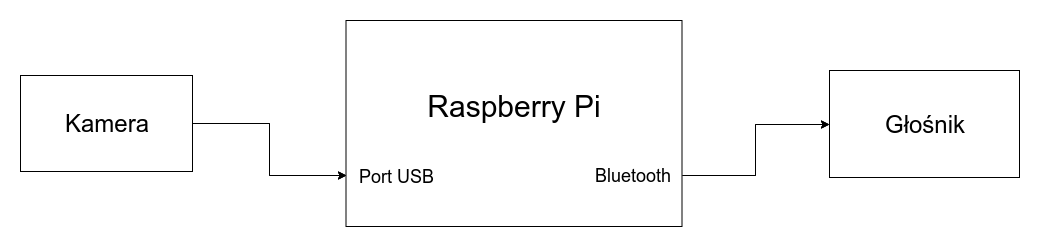
\includegraphics[width=0.9\linewidth]{SW-schematic.png}
	\caption{Schemat połączeń}
	\label{fig:schemat}
\end{figure}
	
\section{Projekt a realizacja}
Aplikacja została napisana w języku Python i Cython. Rozpoznawanie nut zostało zaimplementowane przy użyciu biblioteki OpenCV. Aplikacja jest w stanie rozpoznać nuty z wysoką skutecznością, o ile zdjęcie zostało zrobione w dobrych warunkach oświetleniowych. Algorytm rozpoznaje tylko część symboli - nuty (całe nuty, półnuty, ćwierćnuty i ósemki) oraz klucze. Tą część algorytmu można by rozszerzyć o rozpoznawanie większej ilości symboli. Dokładność rozpoznawania nut również można by ulepszyć na przykład poprzez zastosowanie metod maszynowego uczenia.
	
W trakcie rozwijania projektu dużą przeszkodą była szybkość działania. Dzięki przepisaniu części kodu do języka Cython oraz optymalizacjom aplikacja działa zadowalająco szybko.
	
Pierwotnie w projekcie zakładaliśmy użycie płytki BeagleBone Black. Zdecydowaliśmy się jednak na użycie płytki Raspberry Pi - umożliwiło to proste podłączenie głośnika przez Bluetooth.
	
Aplikacja nie pozwala na wybranie dźwięku instrumentu, co było początkowo planowane. Aplikacja nie odtwarza nut z obu pięciolinii jednocześnie - są odtwarzane po kolei.
	
Aplikację można rozwinąć o lepszy interfejs użytkownika. Obecnie aplikacja jest uruchamiana z linii poleceń. Warto dodać na przykład GUI pokazujące obraz z kamery lub przycisk umożliwiający wykonanie zdjęcia. Brak interfejsu utrudnia ocenę, czy aplikacja działa poprawnie.

\section{Kluczowe fragmenty kodu}
\begin{lstlisting}[language=Python]
#Binaryzacja obrazka - przyjmuje jako input obraz w odcieniach szarości, zwraca obraz czarno biały z uwypuklonymi ciemniejszymi niż tło obszarami. Opiera się na kompletnym zaciemnieniu obszarów, wokół których kolor nigdy się nie zmienia i standardowej binaryzacji dla pozostałych obszarów obrazka

def binarization(bwimg):
	edges = cv.Canny(bwimg,50,150,apertureSize = 3)
	edges2=cv.filter2D(bwimg, -1, kernel[1])
	edges2=cv.Canny(edges2,50,150,apertureSize = 3)
	bwimg=cv.adaptiveThreshold(bwimg, 255, cv.ADAPTIVE_THRESH_GAUSSIAN_C, cv.THRESH_BINARY, Hypers['Binarization_conn'], 1)
	###i wiele linii więcej

#Rotacja obrazka - przyjmuje obraz przed i po binaryzacji, znajduje długie linie na oryginalnym obrazku po czym w zależności od tego, jaki jest w przybliżeniu do 1.8 stopni najczęściej występujący kąt linii, obraca obrazek tak, aby linie znajdujące się pod tym kątem leżały poziomo do obrazka

def rotate_image(img, fimg):
	img2=fimg.copy()
	edges = cv.Canny(img2,50,150,apertureSize = 3)
	lines = cv.HoughLinesP(edges,1,np.pi/180,100,100,10)
	###i wiele linii więcej
	
\end{lstlisting}

\section{Zdjęcia fizycznych połączeń urządzeń}
\begin{figure}[h!]
	\centering
	\begin{subfigure}[b]{0.32\linewidth}
		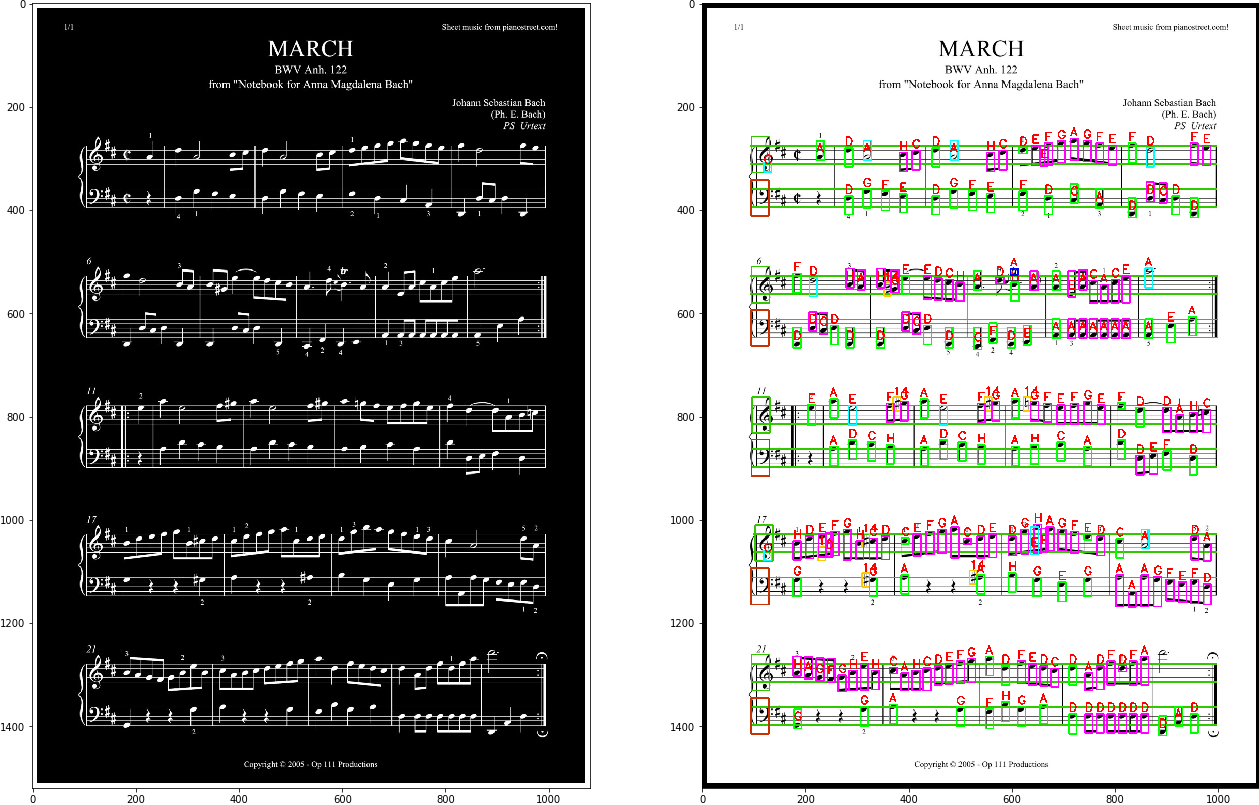
\includegraphics[width=\linewidth]{Zdj0.png}
		\caption{Pierwszy podpis}
	\end{subfigure}
	\begin{subfigure}[b]{0.32\linewidth}
		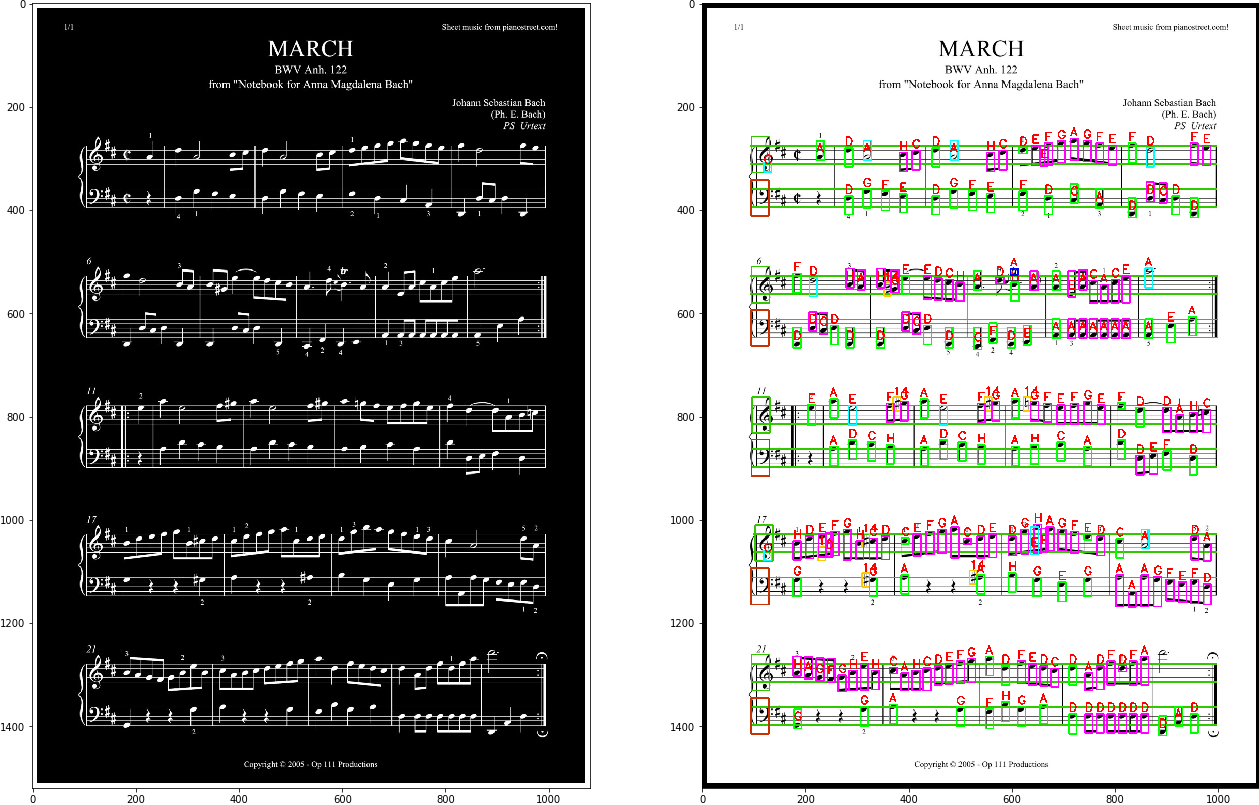
\includegraphics[width=\linewidth]{Zdj0.png}
		\caption{Drugi podpis}
	\end{subfigure}
	\begin{subfigure}[b]{0.32\linewidth}
		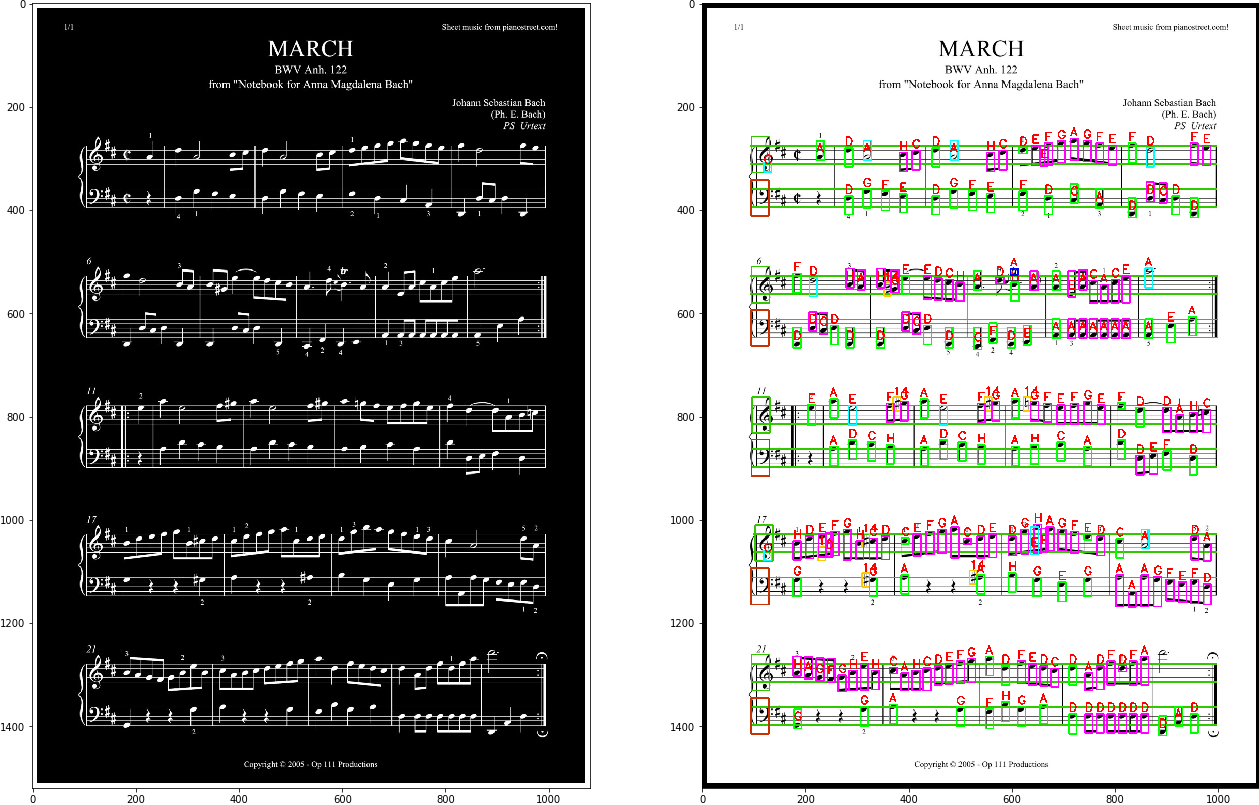
\includegraphics[width=\linewidth]{Zdj0.png}
		\caption{Trzeci podpis}
	\end{subfigure}
	
	\begin{subfigure}[b]{0.48\linewidth}
		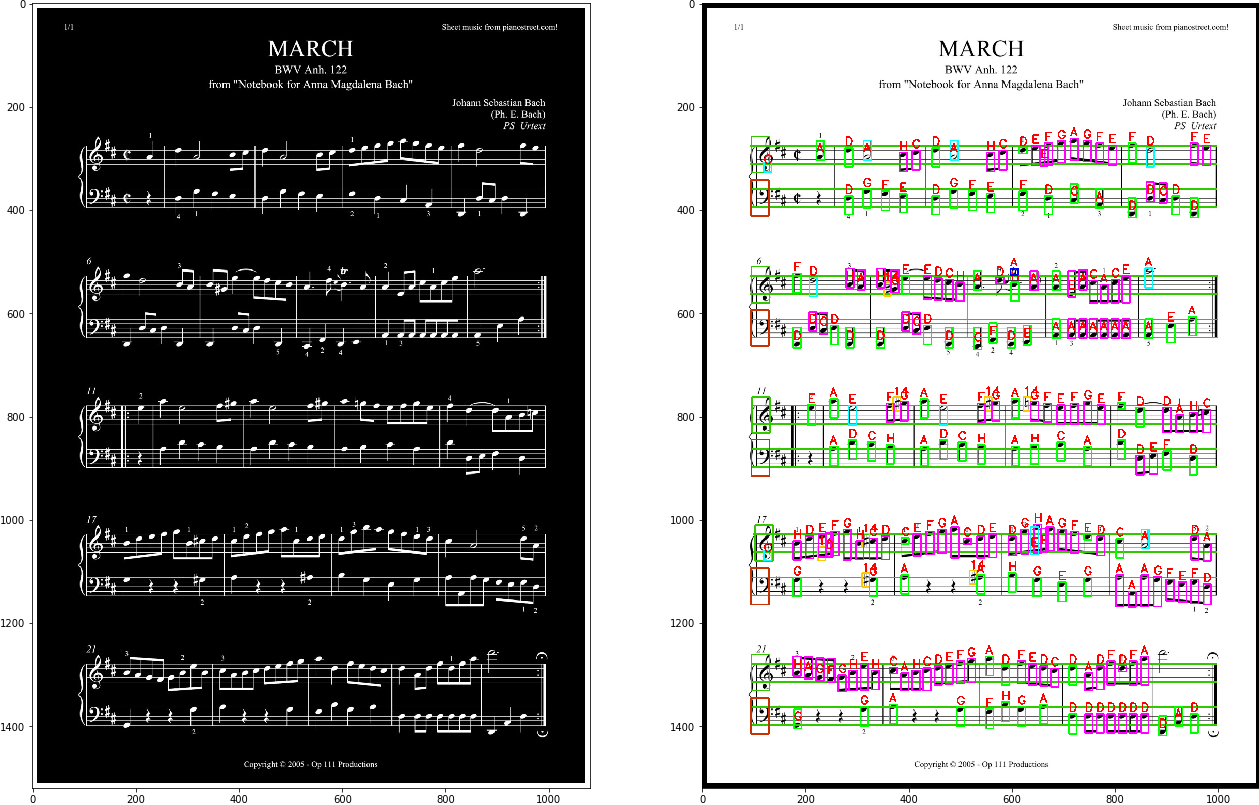
\includegraphics[width=\linewidth]{Zdj0.png}
		\caption{Czwarty podpis}
	\end{subfigure}
	\begin{subfigure}[b]{0.48\linewidth}
		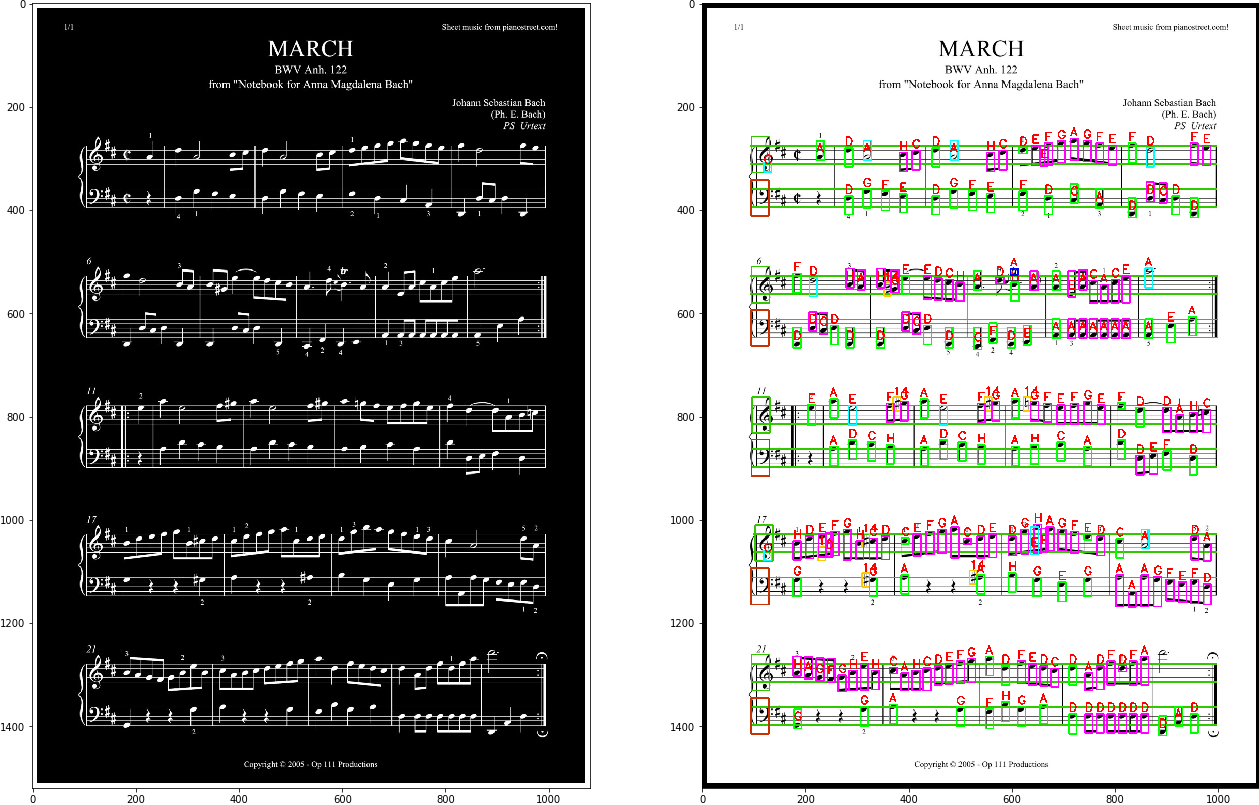
\includegraphics[width=\linewidth]{Zdj0.png}
		\caption{Piąty podpis}
	\end{subfigure}
\end{figure}

\section{Podsumowanie, wnioski}
Aplikacja realizuje swój cel, choć są elementy które można poprawić lub które nie zostały zaimplementowane. Użyty przez nas algorytm uzyskuje wysoką skuteczność przy dobrej jakości zdjęcia; zasadna byłaby próba ulepszenia kodu poprzez użycie metod adaptatywnych, opartych na funkcji kosztu zamiast metod analitycznych przetwarzania obrazu.

\end{document}
